%generare il pdf con il comando: pdflatex main.tex
\documentclass[a4paper, oneside, openany,dvipsnames,table]{article}
\usepackage{../template/sos}
\usepackage{eurosym}
\usepackage{amssymb}% http://ctan.org/pkg/amssymb
\usepackage{pifont}% http://ctan.org/pkg/pifont
\definecolor{bluSOS}{RGB}{48, 84, 150}
\newcommand{\Titolo}{Norme di Progetto}

\newcommand{\Gruppo}{SonsOfSwe}

\newcommand{\Redazione}{Caldart Federico, Cavallin Giovanni, Dalla Riva Giovanni, Favero Andrea, Menegon Lorenzo, Panozzo Stefano, Thiella Eleonora}

\newcommand{\ACapoRedazione}{Caldart Federico \newline Cavallin Giovanni \newline Dalla Riva Giovanni \newline Favero Andrea \newline Menegon Lorenzo \newline Panozzo Stefano \newline Thiella Eleonora}

\newcommand{\Verifica}{Caldart Federico}

\newcommand{\Approvazione}{Cavallin Giovanni}

\newcommand{\Distribuzione}{Vardanega Tullio}

\newcommand{\Uso}{interno}

\newcommand{\Data}{3 Marzo 2018}

\newcommand{\NomeProgetto}{Progetto Speect}

\newcommand{\Mail}{sonsofswe.swe@gmail.com}

\newcommand{\DescrizioneDoc}{Questo documento descrive le regole, gli strumenti e le convenzioni adottate dal gruppo SonsOfSwe durante la realizzazione del progetto Marvin.}



\begin{document}
\copertina{}
%%%%%%%%%%%%%%%%%%%%%%%%%%%%%%%%%%%%%%%%%%%%%%%%%%%%%%%%%%%%%%%%%%%%%%%%%%%%%%%%%%%%%%%%%%%%%%%%%%%%%%%
%SOMMARIO
\definecolor{bluSOS}{RGB}{48, 84, 150}
\definecolor{greySOS}{RGB}{209, 222, 223}
\section*{Registro delle modifiche}
{
	\rowcolors{2}{greySOS}{white}
	\renewcommand{\arraystretch}{1}
	\centering
	\begin{longtable}{| c| c | C{4cm} | c | c |}
		\hline
		\rowcolor{bluSOS}
		\textcolor{white}{\textbf{Versione}} & \textcolor{white}{\textbf{Data}} & \textcolor{white}{\textbf{Descrizione}} & \textcolor{white}{\textbf{Autore}} & \textcolor{white}{\textbf{Ruolo}}\\
		\hline
		1.0.0 & 2018-04--- & Approvazione & Stefano Panozzo  & Reponsabile \\
		\hline
		0.1.0 & 2018-03-10 & Verificazione & Giovanni Cavallin  & Verificatore \\
		\hline
		0.0.1 & 2018-03-07 & Stesura della sezione \emph{Informazioni generali} e \emph{Riassunto della riunione} & Eleonora Thiella & Analista \\
		
	\end{longtable}

}

%\emph{Analisi dei Rischi}, \emph{Preventivo} ed \emph{Attualizzazione dei rischi}. Create le appendici \emph{A Attuazione dei rischi} e \emph{B organigramma}

\newpage
\tableofcontents
\newpage
\listoffigures
\newpage
\listoftables
\newpage
%%%%%%%%%%%%%%%%%%%%%%%%%%%%%%%%%%%%%%%%%%%%%%%%%%%%%%%%%%%%%%%%%%%%%%%%%%%%%%%%%%%%%%%%%%%%%%%%%%%%%%%
%PARAGRAFI
\hypersetup{linkcolor=bluSOS}
\newpage
\section{Introduzione}
\subsection{Scopo del documento}
Questo documento contiene la pianificazione delle attività che saranno svolte dai membri del gruppo \Gruppo{} per realizzare il progetto \NomeProgetto. In particolare, questo documento contiene:

\begin{itemize}
	\item Analisi e trattamento dei rischi;
	\item Il preventivo delle risorse necessarie allo svolgimento del progetto;
	\item Il consuntivo delle attività finora svolte.
\end{itemize}

\subsection{Scopo del prodotto}
Lo scopo del prodotto è quello di realizzare un prototipo di Uniweb come ÐApp che giri su rete Ethereum. I tre attori principali che si rapportano con Marvin sono:
\begin{itemize}
	\item Università;
	\item Professori;
	\item Studenti.
\end{itemize} 
Il portale deve quindi permettere agli studenti di accedere alle informazioni riguardanti le loro carriere universitarie, di iscriversi agli esami, di accettare o rifiutare voti e di poter vedere il loro libretto universitario.
Ai professori deve invece essere permesso registrare i voti degli studenti.
L'università ogni anno crea una serie di corsi di laurea rivolti a studenti, dove ognuno di essi comprende un elenco di esami disponibili per anno accademico. Ogni esame ha un argomento, un numero di crediti e un professore associato. Gli studenti si iscrivono ad un corso di laurea e tramite il libretto elettronico mantengono traccia ufficiale del progresso.

\subsection{Glossario}
Nel documento \textit{Glossario} i termini tecnici, gli acronimi e le abbreviazioni sono definiti in modo chiaro e conciso, in modo tale da evitare ambiguità e massimizzare la comprensione dei documenti.
\newline I vocaboli presenti in esso saranno posti in corsivo e presenteranno una "G" maiuscola a pedice.

\subsection{Riferimenti}
\subsubsection{Normativi}
\begin{itemize}
	\item \textbf{Norme di Progetto: }\textit{Norme di Progetto v1.0.0};
	\item \textbf{Capitolato d'appalto C6: \NomeProgetto}:\\
	\url{http://www.math.unipd.it/~tullio/IS-1/2017/Progetto/C6.pdf};
	\item \textbf{Regolamento del progetto didattico}:\\
	\url{http://www.math.unipd.it/~tullio/IS-1/2017/Dispense/P01.pdf};
	\item \textbf{Vincoli di organigramma e dettagli tecnico-economici}:\\
	\url{http://www.math.unipd.it/~tullio/IS-1/2017/Progetto/RO.html}.
\end{itemize}
\subsubsection{Informativi}
\begin{itemize}
	\item \textbf{Studio di Fattibilità: }\textit{Studio di Fattibilità v1.0.0};
	\item \textbf{Analisi dei Requisiti: }\textit{Analisi dei Requisiti v1.0.0};
	\item \textbf{Software Engineering (10th edition) - Ian Sommerville}:
	\begin{itemize}
		\item Chapter 2: Software processes;
		\item Chapter 22: Project management;
		\item Chapter 23: Project Planning.
	\end{itemize}
	\item \textbf{Slides del corso di Ingegneria del Software}:\\
	\url{http://www.math.unipd.it/~tullio/IS-1/2017/}.
\end{itemize}

\subsection{Modello di sviluppo}
Il modello di sviluppo scelto per il progetto è quello incrementale.\\
Durante i primi periodi, grazie ad un'analisi del capitolato e la comunicazione con il proponente, si fissano i requisiti che il sistema dovrà soddisfare e quali invece sono considerati opzionali, benchè desiderabili. Questo permette di individuare quali dei requisiti hanno una maggior importanza strategica; pertanto questi verranno soddisfatti per primi, mentre gli altri saranno adempiti successivamente.\\
Il modello infatti prevede rilasci multipli successivi, dunque è possibile sottoporre al proponente un prototipo con le funzionalità di primaria importanza nel minor tempo possibile, così da permettere una valutazione in corso d’opera del lavoro svolto. Partendo da questo prototipo sarà poi possibile effettuare un incremento delle funzionalità e un consolidamento di quelle già presenti.\\
Per ottenere ciò nel modo più efficiente ed efficace possibile, si prevede la scomposizione dello sviluppo in attività, al termine delle quali è prevista una milestone (interna o esterna). In questo modo le risorse vengono concentrate in un numero limitato di sottoattività parallele, ottenendo come risultato una loro migliore gestione e verifica.
Questo permette un maggiore controllo sulle tempistiche e sui costi in quanto ogni sottoinsieme deve essere precedentemente pianificato; ciò riduce inoltre il rischio di ritardi.\\
Infine, per ogni attività si prevedono dei giorni di slack prima della consegna dei documenti per accedere alle revisioni di avanzamento, in modo da mitigare eventuali ritardi causati da fattori non prevedibili.

\subsection{Scadenze}\label{Scadenze}
Il gruppo \Gruppo ha deciso di rispettare le seguenti scadenze:
\begin{itemize}
	\item \textbf{Revisione dei Requisiti (RR)}: 23-04-2018;
	\item \textbf{Revisione di Progettazione (RP)}: 14-05-2018;
	\item \textbf{Revisione di Qualifica (RQ)}: 15-06-2018;
	\item \textbf{Revisione di Accettazione (RA)}: 16-07-2018.
\end{itemize}

\section{Obiettivi di qualità}
Questa sezione ha l'obiettivo di definire le caratteristiche riguardanti la qualità di prodotto e di processo che dovranno essere perseguite durante lo sviluppo del progetto.
Ogni caratteristica viene valutata da una metrica, una soglia di accettabilità, ed una possibile soglia di miglioramento che il \emph{team}\ped{G} si prefigge di raggiungere e possibilmente superare.

\subsection{Qualità di processo}
La qualità di processo influenza direttamente il prodotto finale realizzato. É necessario quindi sviluppare un processo in grado di produrre ciclicamente un prodotto di alta qualità. Per questo motivo si è deciso di stabilire le seguenti caratteristiche da rispettare per tutto lo sviluppo del progetto, contemporaneamente a:
\begin{itemize}
\item L'applicazione del \emph{Ciclo di Deming}\ped{G}, o \emph{PDCA}, al fine di perseguire il miglioramento continuo delle attività di processo.
\item L'adesione allo standard ISO/IEC 15504, denominato \emph{SPICE}\ped{G}, al fine di applicare una valutazione oggettiva sulla maturità dei processi.
\end{itemize} 

\subsubsection{Pianificazione}
La pianificazione temporale necessita di uno sguardo a ritroso a partire dagli obiettivi prefissati per completare in tempo adeguato il lavoro previsto. Per un \emph{team}\ped{G} è fondamentale rispettare le scadenze previste, e nel caso in cui si verifichi una situazione di possibile ritardo si rischia di violare l'obiettivo di qualità prefissato, e andranno effettuati quindi dovuti controlli.
\begin{itemize}
	\item \textbf{Metrica}: Si è deciso di utilizzare la \textbf{Schedule Variance}\ped{G}.
	\item \textbf{Soglia di accettabilità}: Si è deciso di ritenere accettabile un ritardo massimo del 10\% rispetto a quanto specificato nel \emph{Piano di Progetto}.
	\item \textbf{Soglia di ottimalità}: Si ritiene un miglioramento rispetto all'obiettivo prefissato il caso in cui un lavoro venga portato a termine in anticipo rispetto a quanto specificato nel \emph{Piano di Progetto}.
\end{itemize}

\subsubsection{Miglioramento}
Al fine di valutare e migliorare la qualità del lavoro svolto è stato assunto il modello di riferimento per la valutazione del livello di maturità definito da SPICE.
\begin{itemize}
	\item \textbf{Metrica}: Verrà utilizzata la struttura a 6 livelli che rappresenta la scala di maturità; la misura di ogni livello sarà effettuata con i 4 livelli N,P,L,F definiti dallo standard.
	\item \textbf{Soglia di accettabilità}: Il livello minimo accettabile di maturità della scala in riferimento ai processi è il 2 (Managed); il processo deve cioè fornire i risultati conformi agli standard ed ai requisiti iniziali in maniera pianificata e tracciabile.
	\item \textbf{Soglia di ottimalità}: La soglia di ottimalità verrà raggiunta con il livello 4 (Predictable); il processo dovrà cioè essere eseguito in conformità ai principi dell'ingegneria del software e attuato all'interno di limiti ben definiti.
\end{itemize}

Per informazioni più approfondite riguardo lo standard ISO/IEC 15504 o SPICE, si rimanda alla sezione~\nameref{AppA:standardProc} dell'appendice A.

\subsubsection{Costo}
Per verificare se i costi sono stati rispettati con quanto concordato nel  \emph{''Piano di Progetto''}, è stato deciso di utilizzare la \emph{\textbf{Cost Variance}}\ped{G} (CV).
Qualora un processo non possieda la qualità minima concordata, necessiterà di lavoro aggiuntivo al fine di soddisfare i requisiti richiesti ma alzando il costo complessivo del progetto, che sarà valutato secondo i seguenti parametri:
\begin{itemize}
	\item \textbf{Metrica}: L'unità di misura scelta per valutare l'aumento dei costi stabiliti è la Cost Variance.
	\item \textbf{Soglia di accettabilità}: Sarà accettabile un aumento dei costi superiore a quelli previsti nel \emph{''Piano di Progetto''} di un massimo del 10\%
	\item \textbf{Soglia di ottimalità}: La soglia di ottimalità verrà raggiunta nel caso in cui i costi non aumenteranno rispetto a quanto concordato nel \emph{''Piano di Progetto''}, 
\end{itemize}

\subsection{Qualità di prodotto}
\subsubsection{Qualità di documento}
Il team si impegna a redigere dei documenti di alta qualità, rispettando le carratestiche di forma e contenuto descritte di seguito.
\paragraph{Ortografia}
Un documento deve essere prima di tutto privo di errori dal punto di vista grammaticale e ortografico. 
Il primo controllo avverà proprio durante la stesura del documento stesso, tramite il sistema di autocontrollo dell'ambiente  \emph{''TexStudio''}, per poi essere controllato una seconda volta dal  \emph{Verificatore}\ped{G}.
\begin{itemize}
	\item \textbf{Metrica}: La quantità di errori riscontrata durante la verifica definitiva del documento sarà l'unità di misura presa in considerazione.
	\item \textbf{Soglia di accettabilità}: Si è accettata come tollerabile la presenza di massimo 3 errori nella seconda e definitiva verifica da parte del \emph{Verificatore}.
	\item \textbf{Sogia di ottimalità}: La soglia di ottimalità verrà raggiunta nel caso in cui dopo la prima revisione del documento non vengano più riscontrati errori dal \emph{Verificatore} e dal \emph{Responsabile}.
\end{itemize}
L'argomento verrà trattato dettagliatamente nella sezione~\nameref{AppB:ErroriOrtografici} in appendice.

\paragraph{Comprensibilità e leggibilità}
Poichè un documento venga considerato leggibile e scorrevole si è deciso di adottare l'\emph{Indice Gulpease}\ped{G}, al fine di avere un parametro oggettivo e facilmente misurabile.
\begin{itemize}
	\item \textbf{Metrica}: L'unità di misura utilizzata è l'\emph{Indice Gulpease}.
	\item \textbf{Soglia di accettabilità}: Verrà considerato come accettabile un valore di 45 sulla scala dell'\emph{Indice Gulpease}.
	\item \textbf{Soglia di ottimalità}: La soglia di ottimalità verrà raggiunta nel caso in cui l'\emph{Indice Gulpease} sia maggiore di 60.
\end{itemize}
L'argomento verrà trattato dettagliatamente nella sezione~\nameref{AppB:IndiceGulpease} in appendice.

\paragraph{Correttezza dei contenuti}
Oltre che ad essere corretto nella forma, un documento necessita di un contenuto adeguato dal punto di vista argomentativo. Gli \emph{Analisti} saranno direttamente responsabili della qualità del contenuto, che poi verrà controllato e corretto dal \emph{Verificatore}.
Per verificare la correttezza concettuale dei documenti prenderemo in esame i seguenti parametri:
\begin{itemize}
	\item \textbf{Metrica}: La quantità di errori di contenuto riscontrata durante la verifica definitiva del documento sarà l'unità di misura presa in considerazione.
	\item \textbf{Soglia di accettabilità}: Si è accettata come tollerabile la presenza di massimo 3 errori nella seconda e definitiva verifica da parte del \emph{Verificatore}.
	\item \textbf{Soglia di ottimalità}: La soglia di ottimalità sarà raggiunta nel caso in cui non si riscontrino errori durante la verifica definitiva del documento.
\end{itemize}

Per maggiori informazioni sulla metrica utilizzata si veda la sezione~\nameref{AppB:ErroriCont} in appendice.

\paragraph{Adesione alle norme interne}
Al fine di ottenere un prodotto coerente ogni documento dovrà essere redatto rispettando strettamente quanto dichiarato nelle \emph{Norme di Progetto}.
Qualunque riferimento non attinente o in contrasto a quanto dichiarato verrà considerato un errore.
\begin{itemize}
	\item \textbf{Metrica}: La quantità di errori di adesione alle norme interne riscontrata durante la verifica definitiva del documento sarà l'unità di misura presa in considerazione. 
	\item \textbf{Soglia di accettabilità}: Si è accettata come tollerabile la presenza di massimo 3 errori nella seconda e definitiva verifica da parte del \emph{Verificatore}.
	\item \textbf{Soglia di ottimalità}: La soglia di ottimalità sarà raggiunta nel caso in cui non si riscontrino errori dopo la prima verifica del documento.
\end{itemize}

Per una precisa definizione degli errori in riferimento alle norme interne si veda la sezione~\nameref{AppB:ErroriForma} in appendice.

\subsubsection{Qualità del software}
Come detto in precedenza, è impossibile distinguere in maniera netta la qualità di processo dalla qualità del software, in quanto la prima influenza direttamente la seconda; è dunque fondamentale avere alla base una qualità di processo sufficientemente buona per garantire la qualità del prodotto. Nonostante ciò, è necessario stabilire degli obiettivi quantitativi di qualità del software oggettivi e misurabili. A tal fine verrà seguito lo standard ISO/IEC 9126, il quale si sostanzia nei sei punti seguenti:

\paragraph{Funzionalità}
È un requisito funzionale che indica la capacità del software di soddisfare le esigenze esposte dal capitolato ed individuate durante l’ \AdR .
Per valutare la funzionalità del software prenderemo in considerazione i seguenti parametri:
\begin{itemize}
	\item \textbf{Metrica}: La valutazione si baserà sul numero di requisiti soddisfatti.
	\item \textbf{Soglia di accettabilità}: Il prodotto verrà valutato come accettabile se tutti i requisiti obbligatori saranno soddisfatti.
	\item \textbf{Soglia di ottimalità}: La soglia di ottimalità sarà raggiunta nel caso in cui siano soddisfatti sia i requisiti obbligatori che tutti i requisiti opzionali.
\end{itemize}

Per maggiori informazioni sulla metrica utilizzata si veda la sezione~\nameref{AppB:Funzionalita} in appendice.


\paragraph{Affidabilità}
È un requisito non funzionale che indica la capacità del software di svolgere correttamente il suo compito, mantenendo delle buone prestazioni anche al variare dell’ambiente nel tempo.
Per valutare l'affidabilità del software prenderemo in considerazione i seguenti parametri:
\begin{itemize}
	\item \textbf{Metrica}: La valutazione si baserà sul numero di fallimenti durante la fase si test.
	\item \textbf{Soglia di accettabilità}: Il prodotto verrà valutato come accettabile se i test falliti saranno inferiori o uguali al 5\%.
	\item \textbf{Soglia di ottimalità}: La soglia di ottimalità sarà raggiunta nel caso in cui il 100\% dei test darà l'esito desiderato.
\end{itemize}

Per maggiori informazioni sulla metrica utilizzata si veda la sezione~\nameref{AppB:Affidabilita} in appendice.

\paragraph{Efficienza}
È un requisito non funzionale che valuta la capacità di un prodotto software di realizzare le funzioni richieste nel minor tempo possibile e con l’uso minimo di risorse necessarie.
\begin{itemize}
	\item \textbf{Metrica}: La valutazione si baserà sui secondi impiegati dal prodotto per eseguire le richieste dell'utente.
	\item \textbf{Soglia di accettabilità}: La soglia di accettabilità è il periodo tra 0 e 10 secondi.
	\item \textbf{Soglia di ottimalità}: La soglia di ottimalità è 1 secondo.
\end{itemize}

Per maggiori informazioni sulla metrica utilizzata si veda la sezione~\nameref{AppB:Efficienza} in appendice.

\paragraph{Usabilità}
L'usabilità è un requisito non funzionale che indica la capacità del software di essere capito e usato correttamente da parte dell'utente finale. Dato che il prodotto finale sarà per l'utente un portale web, è impossibile trovare una metrica quantificabile per valutarne l'usabilità: essa dipende da molteplici fattori che coinvolgono anche le capacità dell'utente stesso e gli strumenti a sua disposizione. Verrà dunque valutata in modo oggettivo basandosi sugli standard del web dichiarati dal \emph{W3C}\ped{G} e sugli strumenti che tale organizzazione mette a disposizione, al fine di creare un'interfaccia web il più accessibile possibile.
Prenderemo in considerazione i seguenti parametri:
\begin{itemize}
	\item \textbf{Metrica}: La valutazione si baserà sul numero di errori trovati dagli strumenti del W3C.
	\item \textbf{Soglia di accettabilità}: La soglia di accettabilità è di 2 errori rilevati.
	\item \textbf{Soglia di ottimalità}: Il prodotto sarà dichiarato ottimo se saranno rilevati 0 errori.
\end{itemize}

Per maggiori informazioni sulla metrica utilizzata si veda la sezione~\nameref{AppB:Usabilita} in appendice.

Quanto detto non assicura però una valutazione completa dell'usabilità, la quale è soggettiva; sarà necessario dunque predisporre test specifici per la misurazione, coinvolgendo ad esempio persone esterne al gruppo al fine di stabilire quanto mediamente il software sia capibile. Al momento il team non è tuttavia in grado di stabilire con precisione una metrica adatta a misurare questo risultato.

\paragraph{Manutenibilità}
La manutenibilità è un requisito non funzionale che indica la capacità di un prodotto di essere evolvibile nel tempo attraverso correzioni, miglioramenti e aggiunte.

\begin{itemize}
\item \textbf{Metrica}: Saranno usate le metriche riguardanti il codice, dato che esso influenza direttamente la manutenibilità del software.
\item \textbf{Soglia di accettabilità}: La soglia di accettabilità sarà raggiunta se il prodotto raggiungerà tale soglia in tutte le metriche utilizzate per il codice.
\item \textbf{Soglia di ottimalità}: La soglia di ottimalità sarà raggiunta se il prodotto raggiungerà tale soglia in tutte le metriche utilizzate per il codice.
\end{itemize}

Per maggiori informazioni sulle metrica per il codice utilizzate si veda la sezione~\nameref{AppB:metricheCod} in appendice.

\paragraph{Portabilità}
La portabilità è un requisito non funzionale che indica la capacità del prodotto di operare in \textit{ambienti}\ped{G} diversi, limitando le necessità di apportare cambiamenti.
\begin{itemize}
	\item Metrica: La valutazione si baserà sul numero di versioni di \emph{browser}\ped{G} e numero di browser stessi su cui il prodotto riesce a venire utilizzato e visualizzato correttamente.
	\item Soglia di accettabilità: La soglia di accettabilità sarà raggiunta se il prodotto sarà supportato correttamente, offrendo la totalità delle sue funzionalità, dalla versione aggiornata dei browser \emph{Google Chrome}\ped{G}, \emph{Microsoft Edge}\ped{G}, \emph{Mozilla Firefox}\ped{G}, \emph{Safari}\ped{G} e \emph{Opera}\ped{G} su \emph{dekstop}\ped{G}.
	\item Soglia di ottimalità: La soglia di ottimalità sarà raggiunta se il prodotto sarà supportato correttamente, offrendo la totalità delle sue funzionalità, in aggiunta ai sopra citati, da \emph{Internet Explorer 11}\ped{G} su desktop e da Google Chrome e Safari nelle versioni \emph{mobile}\ped{G} aggiornate.
\end{itemize}

~\\
Per informazioni più approfondite riguardo lo standard ISO/IEC 9126, si rimanda alla sezione~\nameref{AppA:standardProd} dell'appendice A.




%%%%%%%%%%%%%%%%%%%%%%%%%%%%%%%%%%%%%%%%%%%%%%%%%%%%%%%%%%%%%%%%%%%%%%%%%%%%%%%%%%%%%%%%%%%%%%%%%%%%%%%
\appendix
\pagebreak
\section{Qualità secondo gli standard}
Al fine di perseguire la qualità secondo quanto descritto in questo documento, si è deciso di basarsi su degli standard (descritti qui di seguito) per poter bilanciare la poca esperienza del team con la conoscenza ricavata da anni di pratica nell'ambito dell'ingegneria del software trascritta in tali documenti.
\subsection{Standard di processo: ISO/IEC 15504 - Software Process Improvement and Capability Determination}
\label{AppA:standardProc}
%FONTI:
%http://www.plays-in-business.com/isoiec-15504-spice/
La qualità di un prodotto software dipende dalla qualità dei suoi processi.
L'\emph{ISO/IEC 15504 - Software Process Improvement and Capability Determination} o \emph{SPICE} è uno standard che permette di valutare i processi software di un prodotto con lo scopo di migliorarli  (in modo continuativo). La valutazione dei processi permette di identificare in modo indipendente la \emph{capacità}\ped{G} (capability) di ciascuno di essi attraverso i loro attributi (ovvero gli esiti della valutazione). Basandoci su tali risultati di valutazione (che devono essere comparabili, ripetibili ed oggettivi) ci si può aspettare un miglioramento \emph{continuativo} dei processi e si possono identificare i loro punti di forza, di debolezza ed anche i rischi ed i modi per prevenire questi ultimi.

Ad ogni processo viene assegnato un livello di capacità a seconda della classificazione dei suoi attributi
\begin{labeling}{alligator}
	\item \textbf{0 - Incomplete}: il processo presenta una incapacità generale nel raggiungere il proprio obbiettivo. A questo livello di capacità non viene associato alcun attributo.
	\item \textbf{1 - performed}: il processo è riuscito a raggiungere il proprio obbiettivo. Il raggiungimento di tale obbiettivo potrebbe non essere stato pianificato e tracciato in modo rigoroso. A questo livello è associto l'attributo \textbf{process performance}.
	\item \textbf{2 - managed}: il processo (che appartiene anche al livello 1) rilascia i propri prodotti secondo procedure specifiche ed è pianificato e tracciato. I prodotti sono conformi agli standard specificati ed ai requisiti. A questo livello sono associati due attributi: \textbf{performance management} e \textbf{work product management}.
	\item \textbf{3 - established}: il processo (che appartiene anche al livello 2) viene implementato utilizzando dei buoni principi di ingegneria del software ed è in grado di raggiungere ogni volta che viene eseguito i medesimi risultati. A questo livello sono associati due attributi: \textbf{process definition} e \textbf{process deployment}.
	\item \textbf{4 - predictable}: il processo (che appartiene anche al livello 3) viene eseguito nella pratica in modo coerente rimanendo dentro ai limiti di controllo che, sono stati definiti per raggiungere il suo obbiettivo. Il livello ha associati gli attributi \textbf{process controll} e \textbf{process measurement}
	\item \textbf{5 - optimizing}: le performance del processo (che appartiene anche al livello 4) sono ottimizzate in modo continuo per andare incontro agli obbiettivi ed alle necessità (bisogni) di progetto o di business aziendali presenti e futuri. % I processi raggiungono ''ripetiilità'' nel raggiungere gli obbiettivi di business definiti.
	Anche a questo livello sono associati due attributi: \textbf{process innovation} e \textbf{process optimization}.
\end{labeling}

I 9 attributi che servono per misurare la capacità di un processo sono definiti nel seguente modo:
\begin{labeling}{alligator}
	\item \textbf{Process performance}:  è una misura che indica il raggiungimento degli obbiettivi del processo.
	\item \textbf{Performance management}: è una misura che indica come sono gestite le performance del processo.%The performance management attribute is a measure of the extent to which the performance of the process is managed
	\item \textbf{Work product management}: è una misura che indica quanto i prodotti del processo siano gestiti in modo appropriato.
	\item \textbf{Process definition}: è una misura che indica quanto il processo sia effettivamente impegnato a rispettare gli standard quando produce i propri esiti.
	\item \textbf{Process deployment}: è una misura di quanto il processo standard venga diffuso efficacemente per raggiungere i propri risultati.%The process deployment attribute is a measure of the extent to which the standard process is effectively deployed as a defined process to achieve its process outcomes.
	\item \textbf{Process measurement}:  è una misura che indica quanto vengono usate le misurazioni dei risultati  del processo per assicurarsi che le sue  performance supportino il raggiungimento degli obbiettivi aziendali fissati.
	\item \textbf{Process control}:  è una misura che dà una indicazione di quanto il processo sia gestito in modo quantitativo, questo per produrre un processo che sia stabile, capace\footnote{vedere definizione di \emph{capacità}\ped{G}} e prevedibile entro i limiti definiti.%The process control attribute is a measure of the extent to which the process is quantitatively managed to produce a process that is stable, capable, and predictable within defined limits.
	\item \textbf{Process innovation}: è una misura di quanto i cambiamenti al processo sono identificati grazie ad analisi di cause comuni delle variazioni delle performance e da indagini di approcci innovativi per le definizioni e lo sviluppo dei processi.%The process innovation attribute is a measure of the extent to which changes to the process are identified from analysis of common causes of variation in performance, and from investigations of innovative approaches to the definition and deployment of the process 
	\item \textbf{Process optimization}: è una misura che indica quanto i cambiamenti alla definizione, gestione e performance del processo abbiano un impatto effettivo che permetta di raggiungere gli obiettivi rilevanti di miglioramento del processo.%The process optimization attribute is a measure of the extent to which changes to the definition, management and performance of the process result in effective impact that achieves the relevant process improvement objectives
\end{labeling}

Ogni attributo di processo viene valutato attraverso una scala di valutazione di quattro livelli\footnote{Descritti nella parte 3 dello standard}. Il punteggio è basato sulle prove raccolte tramite degli indicatori che, permettono di sapere in quale livello della classifica si posiziona l'attributo. 
\begin{labeling}{alligator}
	\item \textbf{N - Not achieved}: (0\% - 15\%)
	\item \textbf{P - Partially achieved}: (>15\% - 50\%)
	\item \textbf{L - Largely achieved}: (>50\% - 85\%)
	\item \textbf{F - Fully achieved}: (>85\% - 100\%).
\end{labeling}

Per raggiungere un certo livello di capacità, tutti gli attributi di processo del livello in questione devono essere realizzati almeno come "L" e tutti gli attributi di tutti i livelli di capacità sottostanti devono essere "F".

In Figura~\ref{fig:liv_cap_spice} sono rappresentati gli ultimi cinque livelli di capacità dei processi di SPICE ed i relativi attributi ad essi associati.

\begin{figure}[h!]
	\centering
	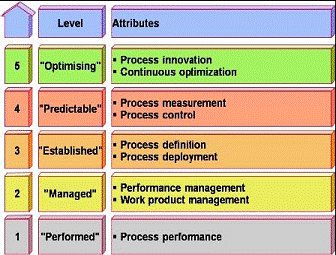
\includegraphics[width=0.50\textwidth]{img/liv_cap_spice.jpg}
	\caption{Ultimi 5 livelli di capacità di SPICE}
	\label{fig:liv_cap_spice}
\end{figure}


\subsection{Standard di prodotto: ISO/IEC 9126}
\label{AppA:standardProd}
Per valutare la qualità del prodotto software si è deciso di utilizzare lo standard ISO/IEC 9126.


É suddiviso in 4 parti:
\begin{labeling}{alligator}
	\item \textbf{Quality Model}: caratteristiche di qualità che possono essere usate per descrivere i fattori di qualità di un prodotto software.
	\item \textbf{External Metrics}: metriche non misurabili direttamente che possono essere usate per valutare se il prodotto software è conforme al modello di qualità.
	\item \textbf{Internal Metrics}: metriche direttamente misurabili utilizzabili per valutare le external metrics.
	\item \textbf{Quality in Use Metrics}: metriche rivolte alla valutazione del sottoinsieme di caratteristiche di qualità legate all’utente.
\end{labeling}

Secondo lo standard sono necessari tre punti di vista per valutare la qualità del prodotto software:
\begin{itemize}
	\item \textbf{percepita/in uso}: è correlata a ciò che percepisce l'utente e per questo motivo definisce delle metriche che possono essere applicate solamente quando il prodotto è finito. Tali metriche esprimono l'efficacia e l'efficienza con cui il software serve le esigenze del suo utilizzatore. 
	 
	\item \textbf{esterna}: rappresenta le prestazioni del prodotto e le funzionalità che esso offre. Definisce delle metriche che esprimono il comportamento dinamico del software, per questo motivo è rilevata attraverso l'analisi dinamica e determina la qualità in uso. É una misura dell'interazione tra il cliente ed il prodotto in un contesto d'uso specifico, permette di osservare il comportamento del software mentre questo viene utilizzato. 
	
	\item \textbf{interna / intrinseca}: rappresenta le qualità intrinseche del prodotto, ovvero quelle misurabili direttamente dal codice sorgente attravero un'analisi di tipo statico. Si realizza partendo dalle specifiche di qualità fornite dall'utente e le specifiche tecniche tradotte dallo sviluppatore nell'architettura del software.
\end{itemize}

Gli attributi di qualità interni, influenzano alcuni degli attributi di qualità esterni e quest'ultimi influenzano quelli della qualità in uso.

Per descrivere i tre punti di vista di cui sopra, lo standard definisce due modelli, uno che riguarda le qualità interna ed esterna, ed un altro che riguarda la qualità in uso. Tali modelli presentano due livelli (primo e secondo) di caratteristiche che definiscono la qualità. Le caratteristiche del secondo livello sono sottocaratteristiche del primo livello e vengono valutate rispetto a delle metriche interne ed esterne. In Figura~\ref{fig:int_ext} e in Figura~\ref{fig:in_use} si possono vedere le caratteristiche associate ai due modelli.

\begin{figure}[h!]
	\centering
	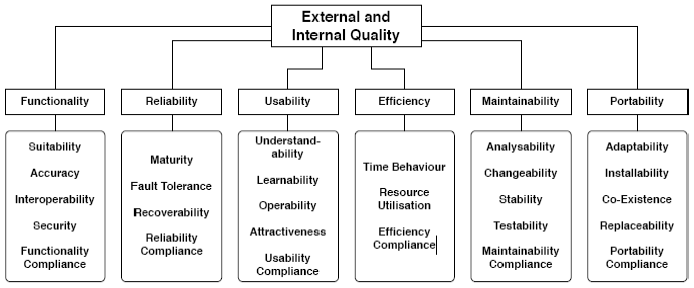
\includegraphics[width=0.50\textwidth]{img/int_ext.png}
	\caption{Caratteristiche associate al modello di qualità interna ed esterna}
	\label{fig:int_ext}
\end{figure}

\begin{figure}[h!]
	\centering
	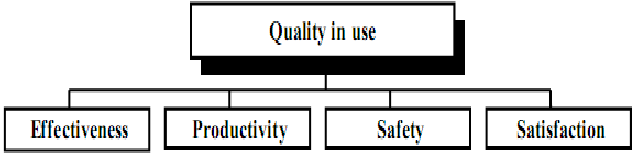
\includegraphics[width=0.50\textwidth]{img/in_use.png}
	\caption{Caratteristiche associate al modello di qualità in uso}
	\label{fig:in_use}
\end{figure}

Di seguito sono elencate le caratteristiche di primo e secondo livello del modello per la qualità interna ed esterna.
\begin{labeling}{alligator}
	\item \textbf{Functionality (funzionalità)}: Il prodotto deve essere in grado di fornire delle funzioni che soddisfino esigenze stabilite (ovvero emerse dall'Analisi dei requisiti).
	\begin{itemize}
		\item \textbf{Suitability (appropriatezza)}: capacità del prodotto di fornire all'utente delle funzioni in grado di soddisfare le esigenze stabilite ed implicite. 
		
		\item \textbf{Accuracy (accuratezza)}: capacità del prodotto di fornire risultati corretti con la precisone richiesta. 
		
		\item \textbf{Interoperability (interoperabilità)}: capacità del prodotto di interagire con uno o più sistemi specificati. 
		
		\item \textbf{Security (sicurezza)}: capacità del prodotto di proteggere i dati e le informazioni in modo che persone/sistemi non autorizzate/i riescano ad accedervi in lettura o scrittura.
		
		\item \textbf{Compliance (conformità)}: capacità del prodotto di aderire agli standard relativi alle funzionalità che offre.
	\end{itemize}
	\item \textbf{Reliability (affidabilità)}: Il prodotto software deve mantenere un livello di prestazioni specificato quando viene eseguito sotto certe condizioni specificate
	\begin{itemize}
		\item \textbf{Maturity (maturità)}: capacità del prodotto di evitare anomalie.
		
		\item \textbf{Fault tolerance (tolleranza all'errore)}: capacità del prodotto di mantenere un livello di prestazioni specificato nel caso occorrano anomalie.
		
		\item \textbf{Recoverability (recuperabilità)}: capacità del prodotto di recuperare un livello di prestazioni specificato ed i dati colpiti da dei malfunzionamenti.
		
		\item \textbf{Compliance (conformità)}: capacità del prodotto di aderire a standard relativi all'affidabilità.
	\end{itemize}
	
	\item \textbf{Usability (usabilità)}: Il prodotto software deve essere compreso ed utilizzato con gradimento dall'utente
	\begin{itemize}
		\item \textbf{Understandability (comprensibilità)}: il prodotto software permette di capire all'utente se può essergli utile per dei compiti particolari.
		
		\item \textbf{Learnability (apprendibilità)}: il prodotto è in grado di far apprendere all'utente come utilizzare le proprie applicazioni.
		
		\item \textbf{Operability (operabilità)}: il prodotto permette all'utente di utilizzarlo e di esercitarne il controllo.
		
		\item \textbf{Attactiveness (attrattività)}: la capacità del prodotto di attrarre l'utente suscitandone un certo livello di gradimento.
		
		\item \textbf{Compliance (conformità)}: la capacità del prodotto di aderire agli standard di usabilità.
	\end{itemize}
	
	\item \textbf{Efficency (efficienza)}: Il prodotto sfrutta al massimo ed al meglio le risorse di cui necessita per espletare le proprie funzioni.
	\begin{itemize}
		\item \textbf{Time behaviour (comportamento nel corso del tempo)}: capacità del prodotto di fornire un tempo di risposta appropriato quando esegue le proprie funzioni.
		
		\item \textbf{Resource utilisation (utilizzo delle risorse)}: la capacità del prodotto di usare la giusta quantità ed il giusto tipo di risorse quando esegue le proprie funzioni.
		
		\item \textbf{Compliance (conformità)}: capacità del prodotto di soddisfare gli standard relativi all'effecienza.
		
	\end{itemize}
	
	\item \textbf{Maintainability (manutenibilità)}: capacità del prodotto di evolversi nel tempo grazie a delle modifiche o correzioni.
	\begin{itemize}
		\item \textbf{Analysability (analizzabilità)}: la capacità del prodotto di essere analizzato per scovare le cause dei malfunzionamenti.
		
		\item \textbf{Changeability (modificabilità)}: la capacità del prodotto di essere modificato.
		
		\item \textbf{Stability (stabilità)}: capacità del software di evitare malfunzionamenti dopo essere stato modificato.
		
		\item \textbf{Testability (testabilità)}: capacità del software modificato di essere verificato e validato.
		
		\item \textbf{Compliance (conformità)}: capacità del prodotto di soddisfare gli standard relativi alla manutenibilità.
	\end{itemize}
	
	\item \textbf{Portability (portabilità)}: Il software deve poter essere trasferito da un ambiente ad un altro con l'avanzare delle nuove tecnologie.
	\begin{itemize}
		\item \textbf{Adaptability (adattabilità)}: la capacità del prodotto di adattarsi ad ambienti diversi senza che ci sia il bisogno di applicare azione alcuna o di utilizzare mezzi diversi da quelli che sono stati già forniti. 
		
		\item \textbf{Installability (instabilità)}: la capacità del prodotto di essere installato in un ambiente specifico.
		
		\item \textbf{Co-existence (coesistenza)}: la capacità del prodotto di coesistere con altri prodotti software indipendenti in uno stesso ambiente condividendone le risorse.
		
		\item \textbf{Replaceability (sostituibilità)}: la capacità del prodotto di sostituire un altro prodotto software con gli stessi scopi nello stesso ambiente. 
		
		\item \textbf{Compliance (conformità)}: capacità del prodotto di soddisfare gli standard relativi alla portabilità.
	\end{itemize}
\end{labeling}

Di seguito sono elencate le caratteristiche del modello per la qualità in uso che, rappresentano il punto di vista dell'utente sulla qualità del prodotto software:

\begin{itemize}
	\item \textbf{Effectiveness (efficacia)}:  permette agli utenti di raggiungere il proprio obbiettivo portandolo a termine con accuratezza e completezza.

	\item \textbf{Productivity (produttività)}: la capacità del prodotto di utilizzare una adeguata quantità di risorse garantendo efficienza.

	\item \textbf{Satisfaction (soddisfazione)}: la capacità del prodotto software di soddisfare gli utenti.

	\item \textbf{Safety (sicurezza)}: la capacità del prodotto di raggiungere livelli accettabili di rischio di danni a persone, software e ambiente operativo su cui è installato.
\end{itemize}

\subsection{Ciclo di Deming}
Il ciclo di Deming, chiamato anche PDCA (Plan, Do, Check, Action.) è uno strumento che permette di realizzare il miglioramento continuo della qualità dei processi e quindi anche dei loro prodotti.

\begin{figure}[h!]
	\centering
	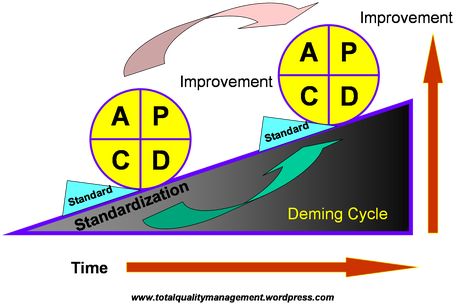
\includegraphics[width=0.50\textwidth]{img/deming.png}
	\caption{Ciclo di Deming}
	\label{fig:PDCA}
\end{figure}

Come si può vedere in Figura~\ref{fig:PDCA} bisogna ripetere in modo iterativo i quattro passi \emph{Plan}, \emph{Do}, \emph{Check} e \emph{Action} per ottenere il miglioramento di un processo.

\begin{itemize}
	\item \textbf{Plan}: vengono pianificati gli obbiettivi per il miglioramento del processo. In questa fase viene analizzata la situazione attuale, vengono raccolti i dati e sviluppate delle metodologie per ottenere dei miglioramenti. Vengono definite le attività che bisogna svolgere, le risorse di cui esse necessitano e si fissano le scadenze.
	
	Per fare ciò è necessario porsi tre domande durante la fase di planning:
	\begin{itemize}
		\item Cosa si sta cercando di realizzare?
		\item Quali cambiamenti si possono fare per ottenere un miglioramento?
		\item Come si è in grado di capire che un dato cambiamento rappresenta un miglioramento?
	\end{itemize}

	\item \textbf{Do}: viene attuato il piano definito nella fase di Plan, in questo modo il processo viene eseguito e così viene creato il prodotto.
	
	\item \textbf{Check}: viene controllato che il processo funzioni come pianificato, in particolare si confrontano i risultati misurati nella fase di Do con gli obbiettivi stabiliti nella fase di Plane (ovvero i risultati attesi).
	
	\item \textbf{Action}: il processo viene migliorato attuando se necessario delle azioni correttive che devono agire sulle differenze riscontrate tra i risultati attesi e quelli misurati.
\end{itemize}

Quando tutte queste quattro fasi vengono portate a termine con il massimo della soddisfazione, il miglioramento viene standardizzato. Il prodotto standardizzato è il risultato dell'iniziativa di miglioramento. É possibile che con il cambiamento di alcune circostanze, il processo sia soggeto ad un nuovo miglioramento, in questo modo il ciclo di deming viene ripetuto di volta in volta.
\pagebreak
\pagebreak
\section{Specifica dei test}
Questa sezione definirà i test che verranno implementati ed eseguiti dal team al fine di garantire, in seguito al loro superamento, la creazione di software di alta qualità che soddisfi le richieste ed aspettative del proponente. 
Ogni test viene riconosciuto tramite un identificativo univoco, la cui sintassi è descritta nelle \NdP (§3.2.2) e può assumere uno tra questi stati: \Ts, \Ti, \Ts. 
Dato che il progetto è ancora alla fase iniziale, si presume che questa sezione sarà soggetta a modifiche basate sulle esigenze ed i problemi che si incontreranno durante lo sviluppo.

\subsection{Test di validazione}
Questi test verranno utilizzati durante la fase di collaudo finale, in presenza di committente e proponente, per valutare se il prodotto è conforme a quanto specificato nel contratto.

\newcolumntype{H}{>{\centering\arraybackslash}m{7cm}}
\normalsize
\begin{longtable}{|c|H|c|}
	\hline
	\textbf{Codice test} & \textbf{Descrizione} & \textbf{Stato}\\
	\hline
	\endhead
	
	\hline
	TV0F1A & Viene verificato che un utente non autenticato visualizzi la pagina di registrazione. & \Ts \\
	\hline
	TV0F1B & Viene verificato l'inserimento nel campo realtivo al nome. & \Ts \\
	\hline
	TV0F1C & Viene verificato l'inserimento nel campo realtivo al cognome. & \Ts \\
	\hline
	TV0F1D & Viene verificato l'inserimento nel campo realtivo all'e-mail. & \Ts \\
	\hline
	TV0F1E & Viene verificato l'inserimento nel campo realtivo al codice fiscale. & \Ts \\
	\hline
	TV0F1F & Viene verificato l'inserimento nel campo realtivo al codice univoco. & \Ts \\
	\hline
	TV0F1G & Viene verificato l'inserimento nel campo realtivo al matricola. & \Ts \\
	\hline
	TV0F1H & Viene verificato che \emph{metamask}\ped{G} sia attivato correttamente nel caso in cui un utente non autenticato voglia registrarsi. & \Ts \\
	\hline
	TV0F1I & Viene verificato che venga confermata la registrazione. & \Ts \\
	\hline
	TV0F1L & Viene verificato che la creazione sia andata a buon fine effettuando un login. & \Ts \\
	\hline
	TV2F1.8 & Viene verificata la visualizzazione di un messaggio d'errore qualora l'utente non autenticato  riempia i campi dato relativi alla registrazione con informazioni già presenti, non valide o nulle. & \Ts \\
	\hline
	TV0F2A & Viene verificato che \emph{metamask}\ped{G} sia attivato correttamente nel caso in cui un utente non autenticato voglia autenticarsi dopo essersi registrato. & \Ts \\
	\hline
	TV0F2B & Viene verificato che, nel caso in cui l'utente non autenticato clicchi il pulsante di login, il sistema segnali la corretta autenticazione. & \Ts \\
	\hline
	TV0F3A & Viene verificato che l'utente amministratore o l'utente università siano correttamente autenticati rispettivamente come amministratore o come università. & \Ts \\ 
	\hline
	TV0F3B & Viene verificata la visualizzazione della pagina per l'inserimento di un anno accademico. & \Ts \\ 
	\hline
	TV0F3C & Viene verificato l'inserimento dell'inizio dell'anno accademico. & \Ts \\ 
	\hline
	TV0F3D & Viene verificato l'inserimento della fine dell'anno accademico. & \Ts \\ 
	\hline
	TV0F3E & Viene verificato l'inserimento della nome dell'anno accademico. & \Ts \\ 
	\hline
	TV0F3F & Viene verificata la conferma dell'aggiunta dell'anno accademico. & \Ts \\ 
	\hline
	TV0F3G & Viene verificato che l'aggiunta dell'anno accademico sia andata a buon fine. & \Ts \\ 
	\hline
	TV2F3.5 & Viene verificata la visualizzazione di un messaggio d'errore qualora l'utente amministratore o università riempiano i campi dato relativi all'inserimento di un anno accademico con informazioni errate o nulle. & \Ts \\
	\hline
	TV0F4A & Viene verificata la visualizzazione della pagina per l'inserimento di un corso di laurea. & \Ts \\
	\hline
	TV0F4B & Viene verificato l'inserimento del codice del corso di laurea. & \Ts \\
	\hline
	TV0F4C & Viene verificato l'inserimento del nome del corso di laurea. & \Ts \\
	\hline
	TV0F4D & Viene verificato l'inserimento della descrizione del corso di laurea. & \Ts \\
	\hline
	TV0F4E & Viene verificato l'inserimento della tipologia del corso di laurea. & \Ts \\
	\hline
	TV0F4G & Viene verificata la conferma dell'aggiunta di un corso di laurea. & \Ts \\
	\hline
	TV0F4H & Viene verificato che l'aggiunta del corso di laurea sia andata a buon fine. & \Ts \\
	\hline
	TV2F4.7 & Viene verificata la visualizzazione di un messaggio d'errore qualora l'utente amministratore o università riempiano i campi dato relativi all'inserimento di un corso di laurea con informazioni errate o nulle. & \Ts \\
	\hline
	TV0F5A & Viene verificata la visualizzazione della pagina per l'inserimento di un'attività didattica. & \Ts \\
	\hline
	TV0F5B & Viene verificato l'inserimento del codice dell'attività didattica. & \Ts \\
	\hline
	TV0F5C & Viene verificato l'inserimento del nome dell'attività didattica. & \Ts \\
	\hline
	TV0F5D & Viene verificato l'inserimento della descrizione dell'attività didattica. & \Ts \\
	\hline
	TV0F5E & Viene verificato l'inserimento del professore associato all'attività didattica. & \Ts \\
	\hline
	TV0F5F & Viene verificato l'inserimento dei crediti dell'attività didattica. & \Ts \\
	\hline
	TV0F5G & Viene verificato l'inserimento del periodo dell'attività didattica. & \Ts \\
	\hline
	TV0F5H & Viene verificata la conferma dell'aggiunta dell'attività didattica. & \Ts \\
	\hline
	TV0F5I & Viene verificato che l'aggiunta dell'attività didattica sia andata a buon fine. & \Ts \\
	\hline
	TV2F5.9 & Viene verificata la visualizzazione di un messaggio d'errore qualora l'utente amministratore o università riempiano i campi dato relativi all'inserimento di un'attività didattica con informazioni errate o nulle. & \Ts \\
	\hline
	TV0F6A & Viene verificata la visualizzazione della pagina per l'inserimento di un esame. & \Ts \\
	\hline
	TV0F6B & Viene verificato l'inserimento del codice dell'esame. & \Ts \\
	\hline
	TV0F6C & Viene verificato l'inserimento della descrizione dell'esame. & \Ts \\
	\hline
	TV0F6D & Viene verificato l'inserimento dell'intervallo di prenotazione dell'esame. & \Ts \\
	\hline
	TV0F6E & Viene verificato l'inserimento della data dell'esame. & \Ts \\
	\hline
	TV0F6F & Viene verificato l'inserimento della tipologia dell'esame. & \Ts \\
	\hline
	TV0F6G & Viene verificato l'inserimento del luogo dell'esame. & \Ts \\
	\hline
	TV0F6H & Viene verificato l'inserimento del professore associato all'esame. & \Ts \\
	\hline
	TV0F6I & Viene verificata la conferma dell'aggiunta dell'esame. & \Ts \\
	\hline
	TV0F6L & Viene verificato che l'aggiunta dell'esame sia andata a buon fine. & \Ts \\
	\hline
	TV2F6.9 & Viene verificata la visualizzazione di un messaggio d'errore qualora l'utente amministratore o università riempiano i campi dato relativi all'inserimento di un'esame con informazioni errate o nulle. & \Ts \\
	\hline
	TV2F11A & Viene verificata la visualizzazione della pagina relativa alla cancellazione di un anno accademico. & \Ts \\
	\hline
	TV2F11B & Viene verificata l'effettiva eleminazione dell'anno accademico qualora l'utente amministratore o l'utente università abbia cliccato sul pulsante di eliminazione. & \Ts \\
	\hline
	TV2F12A & Viene verificata la visualizzazione della pagina relativa alla cancellazione di un corso di laurea. & \Ts \\
	\hline
	TV2F12B & Viene verificata l'effettiva eleminazione del corso di laurea qualora l'utente amministratore o l'utente università abbia cliccato sul pulsante di eliminazione. & \Ts \\
	\hline
	TV2F13A & Viene verificata la visualizzazione della pagina relativa alla cancellazione di un'attività didattica. & \Ts \\
	\hline
	TV2F13B & Viene verificata l'effettiva eleminazione dell'attività didattica qualora l'utente amministratore o l'utente università abbia cliccato sul pulsante di eliminazione. & \Ts \\
	\hline
	TV2F14A & Viene verificata la visualizzazione della pagina relativa alla cancellazione di un'esame. & \Ts \\
	\hline
	TV2F14B & Viene verificata l'effettiva eleminazione dell'esame qualora l'utente amministratore o l'utente università abbia cliccato sul pulsante di eliminazione. & \Ts \\
	\hline
	TV2F16A & Viene verificato che l'utente studente sia correttamente autenticato come studente.  & \Ts \\
	\hline
	TV2F16B & Viene verificata la visualizzazione della pagina della lista di esami associati allo studente.  & \Ts \\
	\hline
	TV2F16C & Viene verificata la conferma dell'iscrizione all'esame da parte dello studente. & \Ts \\
	\hline
	TV2F16D & Viene verificato che l'iscrizione all'esame da parte dello studente sia andata a buon fine. & \Ts \\
	\hline
	TV0F17A & Viene verificato che l'utente professore sia correttamente autenticato come professore.  & \Ts \\
	\hline
	TV0F17B & Viene verificata la visualizzazione della pagina della lista di esami associati al professore.  & \Ts \\
	\hline
	TV0F18 & Viene verificata la visualizzazione della pagina della lista di studenti iscritti ad un esame associato al professore.  & \Ts \\
	\hline
	TV0F23A & Viene verificato l'inserimento di un voto ad uno studente da parte di un professore. & \Ts \\
	\hline
	TV0F23B & Viene verificato che l'inserimento di un voto ad uno studente da parte di un professore sia andato a buon fine. & \Ts \\
	\hline
	TV2F23.3 & Viene verificata la visualizzazione di un messaggio d'errore qualora un professore inserisca un voto in un formato errato. & \Ts \\
	\hline
	TV0F24A & Viene verificata la visualizzazione della pagina relativa all'aggiunta di un nuovo utente da parte di un utente amministratore o di un utente università.  & \Ts \\
	\hline
	TV0F24B & Viene verificato l'inserimento del codice fiscale dell'utente che l'utente amministratore o l'utente università vuole inserire.  & \Ts \\
	\hline
	TV0F24C & Viene verificato l'inserimento del codice univoco dell'utente che l'utente amministratore o l'utente università vuole inserire.  & \Ts \\
	\hline
	TV0F24D & Viene verificata la selezione della tipologia dell'utente che l'utente amministratore o l'utente università vuole inserire.  & \Ts \\
	\hline
	TV0F24E & Viene verificata la selezione dell'anno accademico relativo all'utente che l'utente amministratore o l'utente università vuole inserire.  & \Ts \\
	\hline
	TV0F24F & Viene verificata la selezione del corso di laurea relativa all'utente che l'utente amministratore o l'utente università vuole inserire.  & \Ts \\
	\hline
	TV0F24G & Viene verificata la conferma dell'aggiunta di un nuovo utente da parte di un utente amministratore o di un utente università. & \Ts \\
	\hline
	TV0F24H & Viene verificato che l'aggiunta di un utente da parte di un utente amministratore o di un utente università sia andata a buon fine. & \Ts \\
	\hline
	TV2F24.6 & Viene verificata la visualizzazione di un messaggio d'errore qualora l'utente amministratore o università riempiano i campi dato relativi all'aggiunta di un nuovo utente con informazioni errate o nulle. & \Ts \\
	\hline
	TV0F25A & Viene verificata l'eliminazione di un utente studente da parte dell'utente amministratore o dell'utente università.	& \Ts \\
	\hline
	TV0F25B & Viene verificata l'eliminazione di un utente professore da parte dell'utente amministratore o dell'utente università.	& \Ts \\
	\hline
	TV0F25C & Viene verificata l'eliminazione di un utente amministratore da parte dell'utente università.	& \Ts \\
	\hline
	TV0F26A & Viene verificata la visualizzazione della pagina con la lista di esami a cui lo studente è registrato. & \Ts \\
	\hline
	TV0F26B & Viene verificata la visualizzazione della pagina del libretto universitario da parte dello studente. & \Ts \\
	\hline
	\caption[Test di validazione]{Test di validazione}
	\label{tabella:TV}
\end{longtable}

	\subsubsection{Tracciamento Test di validazione - Requisiti}
\normalsize
\begin{longtable}{|c|c|}
	\hline
	\textbf{Codice test} & \textbf{Codice requisito} \\
	\hline
	\endhead
	TV0F1A & R0F1\\
	\hline
	TV0F1B & R0F1\\
	\hline
	TV0F1C & R0F1\\
	\hline
	TV0F1D & R0F1\\
	\hline
	TV0F1E & R0F1\\
	\hline
	TV0F1F & R0F1\\
	\hline
	TV0F1G & R0F1\\
	\hline
	TV0F1H & R0F1\\
	\hline
	TV0F1I & R0F1\\
	\hline
	TV0F1L & R0F1\\
	\hline
	TV2F1.8 & R2F1.8\\
	\hline
	TV0F2A & R0F2\\
	\hline
	TV0F2B & R0F2\\
	\hline
	TV0F3A & R0F3\\
	\hline
	TV0F3B & R0F3\\
	\hline
	TV0F3C & R0F3\\
	\hline
	TV0F3D & R0F3\\
	\hline
	TV0F3E & R0F3\\
	\hline
	TV0F3F & R0F3\\
	\hline
	TV0F3G & R0F3\\
	\hline
	TV2F3.5 & R2F3.5\\
	\hline
	TV0F4A & R0F4\\
	\hline
	TV0F4B & R0F4\\
	\hline
	TV0F4C & R0F4\\
	\hline
	TV0F4D & R0F4\\
	\hline
	TV0F4E & R0F4\\
	\hline
	TV0F4F & R0F4\\
	\hline
	TV0F4G & R0F4\\
	\hline
	TV0F4H & R0F4\\
	\hline
	TV2F4.7 & R2F4.7\\
	\hline
	TV0F5A & R0F5\\
	\hline
	TV0F5B & R0F5\\
	\hline
	TV0F5C & R0F5\\
	\hline
	TV0F5D & R0F5\\
	\hline
	TV0F5E & R0F5\\
	\hline
	TV0F5F & R0F5\\
	\hline
	TV0F5G & R0F5\\
	\hline
	TV0F5H & R0F5\\
	\hline
	TV0F5I & R0F5\\
	\hline
	TV2F5.9 & R2F5.9\\
	\hline
	TV0F6A & R0F6\\
	\hline
	TV0F6B & R0F6\\
	\hline
	TV0F6C & R0F6\\
	\hline
	TV0F6D & R0F6\\
	\hline
	TV0F6E & R0F6\\
	\hline
	TV0F6F & R0F6\\
	\hline
	TV0F6G & R0F6\\
	\hline
	TV0F6H & R0F6\\
	\hline
	TV0F6I & R0F6\\
	\hline
	TV0F6L & R0F6\\
	\hline
	TV2F6.9 & R2F6.9\\
	\hline
	TV2F11A & R2F11\\
	\hline
	TV2F11B & R2F11\\
	\hline
	TV2F12A & R2F12\\
	\hline
	TV2F12B & R2F12\\
	\hline
	TV2F13A & R2F13\\
	\hline
	TV2F13B & R2F13\\
	\hline
	TV2F14A & R2F14\\
	\hline
	TV2F14B & R2F14\\
	\hline
	TV2F16A & R2F16\\
	\hline
	TV2F16B & R2F16\\
	\hline
	TV2F16C & R2F16\\
	\hline
	TV2F16D & R2F16\\
	\hline
	TV0F17A & R0F17\\
	\hline
	TV0F17B & R0F17\\
	\hline
	TV0F18 & R0F18\\
	\hline
	TV0F23A & R0F23\\
	\hline
	TV0F23B & R0F23\\
	\hline
	TV2F23.3 & R2F23.3\\
	\hline
	TV0F24A & R0F24\\
	\hline
	TV0F24B & R0F24\\
	\hline
	TV0F24C & R0F24\\
	\hline
	TV0F24D & R0F24\\
	\hline
	TV0F24E & R0F24\\
	\hline
	TV0F24F & R0F24\\
	\hline
	TV0F24G & R0F24\\
	\hline
	TV0F24H & R0F24\\
	\hline
	TV2F24.6 & R2F24.6\\
	\hline
	TV0F25A & R0F25\\
	\hline
	TV0F25B & R0F25\\
	\hline
	TV0F25C & R0F25\\
	\hline
	TV0F26A & R0F26\\
	\hline
	TV0F26B & R0F26\\
	\hline
	\caption[Tracciamento test di validazione - requisiti]{Tracciamento test di validazione - requisiti}
\end{longtable}
\clearpage
	
\subsection{Test di sistema}
Questi test servono per verificare il comportamento dinamico complessivo dell'intero sistema in riferimento ai requisiti dichiarati nel documento \AdR, come attività di controllo interna svolta dal fornitore.

\newcolumntype{H}{>{\centering\arraybackslash}m{7cm}}
\normalsize
\begin{longtable}{|c|H|c|}
	\hline
	\textbf{Codice test} & \textbf{Descrizione} & \textbf{Stato}\\
	\hline
	TS0F1 & Viene verificato che il sistema permetta la creazione di un account permettendo di usufruire delle funzionalità del sistema, limitate dal tipo di account creato.& \Ts \\
	\hline
    TS0F2 & Viene verificato che il sistema permetta ad ogni utente correttamente registrato di autenticarsi automaticamente. & \Ts \\
	\hline
	TS0F3 &Viene verificato che il sistema permetta ad ogni utente amministratore o università di aggiungere un nuovo anno accademico al sistema. & \Ts \\ 
	\hline
	TS0F4 & Viene verificato che il sistema permetta ad ogni utente amministratore o università di aggiungere un nuovo corso di laurea al sistema. & \Ts \\
	\hline
	TS0F5 & Viene verificato che il sistema permetta ad ogni utente amministratore o università di aggiungere una nuova attività didattica al sistema. & \Ts \\
	\hline
	TS0F6 &  Viene verificato che il sistema permetta ad ogni utente amministratore o università di aggiungere un nuovo esame al sistema. & \Ts \\
	\hline
	TS2F11 & Viene verificato che il sistema permetta ad ogni utente amministratore o università di eliminare un anno accademico già presente nel sistema. & \Ts \\
	\hline
	TS2F12 & Viene verificato che il sistema permetta ad ogni utente amministratore o università di eliminare un corso di laurea già presente nel sistema. & \Ts \\
	\hline
	TS2F13 & Viene verificato che il sistema permetta ad ogni utente amministratore o università di eliminare un'attività didattica già presente nel sistema. & \Ts \\
	\hline
	TS2F14 & Viene verificato che il sistema permetta ad ogni utente amministratore o università di eliminare un esame già presente nel sistema. & \Ts \\
	\hline
	TS2F15 &Viene verificato che il sistema permetta ad ogni utente amministratore o università di inserire un nuovo professore associato ad un'attività didattica. & \Ts \\
	\hline
	TS2F16 & Viene verificato che il sistema permetta ad ogni utente studente di iscriversi ad un esame.& \Ts \\
	\hline
	TS0F17 & Viene verificato che il sistema permetta ad ogni utente professore di visualizzare la lista degli esami a lui associati. & \Ts \\
	\hline
	TS0F18 & Viene verificato che il sistema permetta ad ogni utente professore di visualizzare la lista degli studenti iscritti ad uno degli esami a lui associati. & \Ts \\
	\hline
	TS0F19 & Viene verificato che il sistema visualizzi per ogni operazione il costo associato. & \Ts \\
	\hline
	TS0F23 & Viene verificato che il sistema permetta ad ogni utente professore di registrare il voto relativo ad un esame di uno studente. & \Ts \\
	\hline
	TS0F24 & Viene verificato che il sistema permetta ad ogni utente amministratore o università di creare un nuovo utente nel sistema.& \Ts \\
    \hline
	TS0F25 & Viene verificato che il sistema permetta ad ogni utente amministratore o università di rimuovere un utente dal sistema. & \Ts \\
	\hline
	TS0F26 & Viene verificato che il sistema permetta ad ogni utente studente di visualizzare il proprio libretto. & \Ts \\
	\hline
	TS &  Viene verificato che il sistema offra correttamente tutte le sue funzionalità con la versione 6.0.286 o superiore di Google Chrome, utilizzando metamask versione 4.6 o superiore.  & \Ts \\
	\hline
	TS &   Viene verificato che il sistema offra correttamente tutte le sue funzionalità con la versione 50 o superiore di Mozilla Firefox, utilizzando metamask versione 4.5 o superiore. & \Ts \\
	\hline
	TS &   Viene verificato che il sistema offra correttamente tutte le sue funzionalità con la versione 52 o superiore di Opera, utilizzando metamask versione 3.13.4 o superiore. & \Ts \\
	\hline
	\caption[Test di sistema]{Test di sistema}
\end{longtable}
\clearpage

\subsubsection{Tracciamento Test di sistema - Requisiti}
\normalsize
\begin{longtable}{|c|c|}
	\hline
	\textbf{Codice test} & \textbf{Codice requisito} \\
	\hline
	\endhead
	TS0F1 & R0F1\\
	\hline
	TS0F2 & R0F2\\
	\hline
	TS0F3 & R0F3\\
	\hline
	TS0F4 & R0F4\\
	\hline
	TS0F5 & R0F5\\
	\hline
	TS0F6 & R0F6\\
	\hline
	TS2F11 & R2F11\\
	\hline
	TS2F12 & R2F12\\
	\hline
	TS2F13 & R2F13\\
	\hline
	TS2F14 & R2F14\\
	\hline
	TS2F15 & R2F15\\
	\hline
	TS2F16 & R2F16\\
	\hline
	TS0F17 & R0F17\\
	\hline
	TS0F18 & R0F18\\
	\hline
	TS0F19 & R0F19\\
	\hline
	TS0F23 & R0F23\\
	\hline
	TS0F24 & R0F24\\
	\hline
	TS0F25 & R0F25\\
	\hline
	TS0F26 & R0F26\\
	\hline
	TS0F27 & R0F27\\
	\hline
	TS0F28 & R0F28\\
	\hline
	\caption[Tracciamento test di sistema - requisiti]{Tracciamento test di sistema - requisiti}
\end{longtable}
\clearpage

\subsection{Test di integrazione}
Questi test verificano il corretto comportamento di ogni singola componente e le relazioni con il resto del sistema.

\newcolumntype{H}{>{\centering\arraybackslash}m{7cm}}
\normalsize
\begin{longtable}{|c|H|c|}
	\hline
	\textbf{Codice test} & \textbf{Descrizione} & \textbf{Stato}\\
	\hline
	TI1 & Viene verificato che l’applicazione Web gestisca correttamente il front end del prodotto e le sue interazioni con il back end. & \Ts \\
	\hline
	TI2 & Viene verificato che i contratti Solidity si integrino correttamente con la componente web3. & \Ts \\ 
	\hline
	TI3 & Viene verificato che le componenti \emph{action}, \emph{store} e \emph{reducers} di Redux comunichino correttamente tra loro.  & \Ts \\
	\hline
	TI4 & Viene verificato che le componenti visive di React si integrino correttamente con la gestione degli \emph{state} di Redux. & \Ts \\
	\hline
	TI5 & Viene verificato che l'immissione dei dati nel front end corrisponda ad una loro effettiva scrittura nel database del back end. & \Ts \\
	\hline
	TI6 &Viene verificato che l'applicativo web mostri correttamente i dati prelevati dal back end. & \Ts \\ 
	\hline
		\caption[Test di integrazione]{Test di integrazione}
\end{longtable}
\clearpage

\subsection{Test di unità}
Questi test servono per verificare il corretto funzionamento delle singole parti del sistema.

\newcolumntype{H}{>{\centering\arraybackslash}m{7cm}}
\normalsize
\begin{longtable}{|c|H|c|}
	\hline
	\textbf{Codice test} & \textbf{Descrizione} & \textbf{Stato}\\
	\hline
	TU1 & Viene verificato che il metodo \emph{LogoutUser()} faccia uscire l'utente dal sistema e faccia il dispatch dello stato dell'operazione. & \Ts \\
	\hline
	TU2 & Viene verificato che il metodo \emph{OnInsertUserFormSubmit(string,string,int)} inserisca un utente nel sistema e faccia il dispatch dello stato dell'operazione. & \Ts \\
	\hline
	TU3 &Viene verificato che dopo aver aggiunto un utente al sistema, esso sia effettivamente salvato nella blockchain assieme al suo codice univoco e codice fiscale. & \Ts \\ 
	\hline
	TU4 & Viene verificato che, dopo che un utente ha eseguito la registrazione tramite il codice univoco fornito dall'università ed il suo codice fiscale, immettendo i propri dati personali, esso risulti effettivamente registrato con i propri dati salvati. & \Ts \\
	\hline
	TU5 & Viene verificato che l'inserimento di un nuovo anno accademico sia effettivamente salvato con i dati relativi specificati. & \Ts \\
	\hline
	TU6 &  Viene verificato che l'inserimento di un nuovo corso di laurea sia effettivamente salvato con i dati relativi specificati. & \Ts \\
	\hline
	TU7 & Viene verificato che l'inserimento di un nuovo esame sia effettivamente salvato con i dati relativi specificati. & \Ts \\ 
	\hline
	TU8 & Viene verificato che l'associazione di un esame con un professore comporti effettivamente un collegamento tra le due parti.  & \Ts \\
	\hline
	TU9 & Viene verificato che il metodo \emph{RemoveAdmic(admin)} rimuova correttamente le informazioni e faccia il dispatch dello stato dell'operazione. & \Ts \\
	\hline
	TU10 & Viene verificato che il metodo \emph{RemoveStudent(student)} rimuova correttamente le informazioni e faccia il dispatch dello stato dell'operazione. & \Ts \\
	\hline
	TU11 & Viene verificato che il metodo \emph{ViewStudentList(exam)} visualizzi correttamente le informazioni e faccia il dispatch dello stato dell'operazione. & \Ts \\
	\hline
	TU12 & Viene verificato che il metodo \emph{LoginUser()} autentichi correttamente l'utente nel sistema e faccia il dispatch dello stato dell'operazione. & \Ts \\
	\hline
	TU13 & Viene verificato che il metodo \emph{render()} del component \emph{Help} comporti la corretta renderizzazione del componente. & \Ts \\
	\hline
	TU14 & Viene verificato che il metodo \emph{render()} del component \emph{LoginButoon} comporti la corretta renderizzazione del componente. & \Ts \\
	\hline
	TU15 & Viene verificato che il metodo \emph{render()} del component \emph{LogoutButton} comporti la corretta renderizzazione del componente. & \Ts \\
	\hline
	TU16 & Viene verificato che il metodo \emph{render()} del component \emph{NavButton} comporti la corretta renderizzazione del componente. & \Ts \\
	\hline
	TU17 & Viene verificato che il metodo \emph{render()} del component \emph{Home} comporti la corretta renderizzazione del componente. & \Ts \\
	\hline
	TU18 & Viene verificato che il metodo \emph{render()} del component \emph{App} comporti la corretta renderizzazione del componente. & \Ts \\
	\hline
	TU19 & Viene verificato che il metodo \emph{render()} del component \emph{InsertUserForm} comporti la corretta renderizzazione del componente. & \Ts \\
	\hline
	TU20 & Viene verificato che il metodo \emph{render()} del component \emph{InsertUser} comporti la corretta renderizzazione del componente. & \Ts \\
	\hline
	TU21 & Viene verificato che il metodo \emph{render()} del component \emph{EmptyData} comporti la corretta renderizzazione del componente. & \Ts \\
	\hline
	TU22 & Viene verificato che il metodo \emph{render()} del component \emph{DeleteAdministrator} comporti la corretta renderizzazione del componente. & \Ts \\
	\hline
	TU23 & Viene verificato che il metodo \emph{render()} del component \emph{Administrators} comporti la corretta renderizzazione del componente. & \Ts \\
	\hline
	TU24 & Viene verificato che il metodo \emph{render()} del component \emph{LoadingData} comporti la corretta renderizzazione del componente. & \Ts \\
	\hline
	TU25 & Viene verificato che il metodo \emph{render()} del component \emph{LoadingUser} comporti la corretta renderizzazione del componente. & \Ts \\
	\hline
	TU26 & Viene verificato che il metodo \emph{render()} del component \emph{NotFound} comporti la corretta renderizzazione del componente. & \Ts \\
	\hline
	TU27 & Viene verificato che il metodo \emph{render()} del component \emph{ModifyAcademicYear} comporti la corretta renderizzazione del componente. & \Ti \\
	\hline
	TU28 & Viene verificato che il metodo \emph{render()} del component \emph{InsertAcademicYear} comporti la corretta renderizzazione del componente. & \Ts \\
	\hline
	TU29 & Viene verificato che il metodo \emph{render()} del component \emph{DeleteAcademicYear} comporti la corretta renderizzazione del componente. & \Ti \\
	\hline
	TU30 & Viene verificato che il metodo \emph{render()} del component \emph{AcademicYears} comporti la corretta renderizzazione del componente. & \Ts \\
	\hline
	TU31 & Viene verificato che il metodo \emph{render()} del component \emph{ModifyDegreeCourse} comporti la corretta renderizzazione del componente. & \Ti \\
	\hline
	TU32 & Viene verificato che il metodo \emph{render()} del component \emph{InsertDegreeCourse} comporti la corretta renderizzazione del componente. & \Ts \\
	\hline
	TU33 & Viene verificato che il metodo \emph{render()} del component \emph{DeleteDegreeCourse} comporti la corretta renderizzazione del componente. & \Ti \\
	\hline
	TU34 & Viene verificato che il metodo \emph{render()} del component \emph{DegreeCourses} comporti la corretta renderizzazione del componente. & \Ts \\
	\hline
	TU35 & Viene verificato che il metodo \emph{render()} del component \emph{ModifyDidacticActivity} comporti la corretta renderizzazione del componente. & \Ti \\
	\hline
	TU36 & Viene verificato che il metodo \emph{render()} del component \emph{InsertDidacticActivity} comporti la corretta renderizzazione del componente. & \Ts \\
	\hline
	TU37 & Viene verificato che il metodo \emph{render()} del component \emph{DeleteDidacticActivity} comporti la corretta renderizzazione del componente. & \Ti \\
	\hline
	TU38 & Viene verificato che il metodo \emph{render()} del component \emph{DidacticActivities} comporti la corretta renderizzazione del componente. & \Ts \\
	\hline
	TU39 & Viene verificato che il metodo \emph{render()} del component \emph{InsertExam} comporti la corretta renderizzazione del componente. & \Ts \\
	\hline
	TU40 & Viene verificato che il metodo \emph{render()} del component \emph{DeleteProfessor} comporti la corretta renderizzazione del componente. & \Ti \\
	\hline
	TU41 & Viene verificato che il metodo \emph{render()} del component \emph{Professors} comporti la corretta renderizzazione del componente. & \Ts \\
	\hline
	TU42 & Viene verificato che il metodo \emph{render()} del component \emph{DeleteStudent} comporti la corretta renderizzazione del componente. & \Ts \\
	\hline
	TU43 & Viene verificato che il metodo \emph{render()} del component \emph{Students} comporti la corretta renderizzazione del componente. & \Ts \\
	\hline
	TU44 & Viene verificato che il metodo \emph{render()} del component \emph{ExamList} comporti la corretta renderizzazione del componente. & \Ts \\
	\hline
	TU45 & Viene verificato che il metodo \emph{render()} del component \emph{ExamPage} comporti la corretta renderizzazione del componente. & \Ts \\
	\hline
	TU46 & Viene verificato che il metodo \emph{render()} del component \emph{ExamsProfessorList} comporti la corretta renderizzazione del componente. & \Ts \\
	\hline
	TU47 & Viene verificato che il metodo \emph{render()} del component \emph{RegisteredStudentsList} comporti la corretta renderizzazione del componente. & \Ts \\
	\hline
	TU48 & Viene verificato che il metodo \emph{render()} del component \emph{ExamsStudentList} comporti la corretta renderizzazione del componente. & \Ts \\
	\hline
	TU49 & Viene verificato che il metodo \emph{render()} del component \emph{SchoolRecords} comporti la corretta renderizzazione del componente. & \Ts \\
	\hline
	TU50 & Viene verificato che il metodo \emph{render()} del component \emph{Profile} comporti la corretta renderizzazione del componente. & \Ts \\
	\hline
	TU51 & Viene verificato che il metodo \emph{render()} del component \emph{SubNavbar} comporti la corretta renderizzazione del componente. & \Ts \\
	\hline
	TU52 & Viene verificato che il metodo \emph{render()} del component \emph{SubNavButton} comporti la corretta renderizzazione del componente. & \Ts \\
	\hline
	TU53 & Viene verificato che il metodo \emph{render()} del component \emph{SignUp} comporti la corretta renderizzazione del componente. & \Ts \\
	\hline
	TU54 & Viene verificato che il metodo \emph{render()} del component \emph{SignUpForm} comporti la corretta renderizzazione del componente. & \Ts \\
	\hline
	TU55 & Viene verificato che il metodo \emph{ReadAcademicData()} legga correttamente le informazioni e faccia il dispatch dello stato dell'operazione. & \Ts \\
	\hline
	TU56 & Viene verificato che il metodo \emph{ReadDidacticActivities(int,int)} legga correttamente le informazioni e faccia il dispatch dello stato dell'operazione. & \Ts \\
	\hline
	TU57 & Viene verificato che il metodo \emph{ReadDegreeCourses(int)} legga correttamente le informazioni e faccia il dispatch dello stato dell'operazione. & \Ts \\
	\hline
	TU58 & Viene verificato che il metodo \emph{ReadExams(int,int,int)} legga correttamente le informazioni e faccia il dispatch dello stato dell'operazione. & \Ts \\
	\hline
	TU59 & Viene verificato che il metodo \emph{ReadProfessorList()} legga correttamente le informazioni e faccia il dispatch dello stato dell'operazione. & \Ts \\
	\hline
	TU60 & Viene verificato che il metodo \emph{ReadAdminList()} legga correttamente le informazioni e faccia il dispatch dello stato dell'operazione. & \Ts \\
	\hline
	TU61 & Viene verificato che il metodo \emph{ReadStudentsList()} legga correttamente le informazioni e faccia il dispatch dello stato dell'operazione. & \Ts \\
	\hline
	TU62 & Viene verificato che il metodo \emph{ReadExam(int,int,int)} legga correttamente le informazioni e faccia il dispatch dello stato dell'operazione. & \Ts \\
	\hline
	TU63 & Viene verificato che il metodo \emph{ReadExamList(professor)} legga correttamente le informazioni e faccia il dispatch dello stato dell'operazione. & \Ts \\
	\hline
	TU64 & Viene verificato che il metodo \emph{ReadExamList(student)} legga correttamente le informazioni e faccia il dispatch dello stato dell'operazione. & \Ts \\
	\hline
	TU65 & Viene verificato che il metodo \emph{ModifyAcademicData()} modifichi correttamente le informazioni e faccia il dispatch dello stato dell'operazione. & \Ts \\
	\hline
	TU66 & Viene verificato che il metodo \emph{ModifyDidacticActivity(int,int,int)} modifichi correttamente le informazioni e faccia il dispatch dello stato dell'operazione. & \Ts \\
	\hline
	TU67 & Viene verificato che il metodo \emph{ModifyDegreeCourse(int,int)} modifichi correttamente le informazioni e faccia il dispatch dell'operazione. & \Ts \\
	\hline
	TU68 & Viene verificato che il metodo \emph{ModifyExam(int,int,int,int)} modifichi correttamente le informazioni e faccia il dispatch dell'operazione. & \Ts \\
	\hline
	TU69 & Viene verificato che il metodo \emph{OnSignUpFormSubmit(string,string,string,string,int)} inserisca un utente nel sistema registrandone i dati nel sistema e faccia il dispatch dello stato dell'operazione. & \Ts \\
	\hline
	TU70 & Viene verificato che il metodo \emph{AddAcademicYear(int)} aggiunga correttamente le informazioni e faccia il dispatch dello stato dell'operazione. & \Ts \\
	\hline
	TU71 & Viene verificato che il metodo \emph{AddDidacticActivity(int,int,int)} aggiunga correttamente le informazioni e faccia il dispatch dello stato dell'operazione. & \Ts \\
	\hline
	TU72 & Viene verificato che il metodo \emph{AddDegreeCourse(int,int)} aggiunga correttamente le informazioni e faccia il dispatch dello stato dell'operazione. & \Ts \\
	\hline
	TU73 & Viene verificato che il metodo \emph{AddExam(int,int,int,int)} aggiunga correttamente le informazioni e faccia il dispatch dello stato dell'operazione. & \Ts \\
	\hline
	TU74 & Viene verificato che il metodo \emph{RemoveAcademicYear(int)} rimuova correttamente le informazioni e faccia il dispatch dello stato dell'operazione. & \Ts \\
	\hline
	TU75 & Viene verificato che il metodo \emph{RemoveDidacticActivity(int,int,int)} rimuova correttamente le informazioni e faccia il dispatch dello stato dell'operazione. & \Ts \\
	\hline
	TU76 & Viene verificato che il metodo \emph{RemoveDegreeCourse(int,int)} rimuova correttamente le informazioni e faccia il dispatch dello stato dell'operazione. & \Ts \\
	\hline
	TU77 & Viene verificato che il metodo \emph{RemoveExam(int,int,int,int)} rimuova correttamente le informazioni e faccia il dispatch dello stato dell'operazione. & \Ts \\
	\hline
	TU78 & Viene verificato che il metodo \emph{RemoveProfessor(admin)} rimuova correttamente le informazioni e faccia il dispatch dello stato dell'operazione. & \Ts \\
	\hline

	\caption[Test di sistema]{Test di sistema}
\end{longtable}

\subsubsection{Tracciamento Test di unità - Metodi}
\normalsize
\begin{longtable}{|>{\centering\arraybackslash}p{2cm}| p{15cm}|}
	\hline
	\textbf{Codice test} & \textbf{Classe:metodo} \\
	\hline
	\endhead
	TU1 & $InsertUserFormAction:OnInsertUserFormSubmit(string,string,int)$ \\
	\hline
	TU2 & $LogoutButtonAction:LogoutUser()$ \\
	\hline
	TU3 & $Admin:addUser(bytes32 \textunderscore fiscalCode, bytes10 \textunderscore uniCode, uint8 \textunderscore userType)$\newline$UserData:getUsersUniCode(bytes32 \textunderscore fiscalCode)$\newline$UserData:getUsersUserType(bytes32 \textunderscore fiscalCode)$
	\\
	\hline

	TU4 & $UserLogic:signUp(bytes32 \textunderscore fiscalCode, bytes10 \textunderscore uniCode, bytes32 \textunderscore hashData)$\newline$UserData:getRegUsersUniCode(address \textunderscore address) $\newline$UserData:getRegUsersFiscalCode(address \textunderscore address)$\newline$UserData:getRegUsersUserType(address \textunderscore address) $\newline$UserData:getRegUsersBadgeNumber(address \textunderscore address)$\newline$UserData:getRegUsersHashData(address \textunderscore address)$\\
	\hline
	TU5 & $Admin:addNewDegree(bytes10 \textunderscore degreeUniCode, bytes4 \textunderscore year, bytes32 \textunderscore hashData) $\newline$DegreeData:isDegree(bytes10 \textunderscore degreeUniCode) $\newline$DegreeData:getDegreeCourses(bytes10 \textunderscore degreeUniCode)$\\
	\hline
	TU6 &$Admin:addNewExam(bytes10 \textunderscore courseUniCode, bytes10 \textunderscore examUniCode, uint32 \textunderscore examTeacher,$\newline$ bytes32 \textunderscore examHashData) $\newline$ExamData:examExist(bytes10 \textunderscore examUniCode)$\newline$ExamData:getExamTeacher(bytes10 \textunderscore examUniCode) $\newline$ExamData:getAllIdentifiers()$\\
	\hline
	TU7 & $Teacher:myExams()$\\
	\hline
	TU8 &$ Teacher:registerResult(bytes10 \textunderscore examUniCode, uint32 \textunderscore studentBadgeNumber, bytes2 \textunderscore result)$\\
	\hline
	TU9 & $DeleteAdministrator:RemoveAdmin(admin)$\\
	\hline
	TU10 & $DeleteStudent:RemoveStudent(steudent)$\\
	\hline
	TU11 & $RegisteredStudentListAction:ViewStudentListAction(exam)$\\
	\hline
	TU12 & $LoginButtonAction:LoginUser()$\\
	\hline
	TU13 & $Help:render$\\
	\hline
	TU14 & $LoginButton:render$\\
	\hline
	TU15 & $LogoutButton:render$\\
	\hline
	TU16 & $NavButton:render$\\
	\hline
	TU17 & $Home:render$\\
	\hline
	TU18 & $App:render$\\
	\hline
	TU19 & $InsertUserForm:render$\\
	\hline
	TU20 & $InsertUser:render$\\
	\hline
	TU21 & $EmptyData:render$\\
	\hline
	TU22 & $DeleteAdministrator:render$\\
	\hline
	TU23 & $Administrators:render$\\
	\hline
	TU24 & $LoadingData:render$\\
	\hline
	TU25 & $LoadingUser:render$\\
	\hline
	TU26 & $NotFound:render$\\
	\hline
	TU27 & $ModifyAcademicYear:render$\\
	\hline
	TU28 & $InsertAcademicYear:render$\\
	\hline
	TU29 & $DeleteAcademicYear:render$\\
	\hline
	TU30 & $AcademicYears:render$\\
	\hline
	TU31 & $ModifyDegreeCourse:render$\\
	\hline
	TU32 & $InsertDegreeCourse:render$\\
	\hline
	TU33 & $DeleteDegreeCourse:render$\\
	\hline
	TU34 & $DegreeCourses:render$\\
	\hline
	TU35 & $ModifyDidacticActivity:render$\\
	\hline
	TU36 & $InsertDidacticActivity:render$\\
	\hline
	TU37 & $DeleteDidacticActivity:render$\\
	\hline
	TU38 & $DidacticActivities:render$\\
	\hline
	TU39 & $InsertExam:render$\\
	\hline
	TU40 & $DeleteProfessor:render$\\
	\hline
	TU41 & $Professors:render$\\
	\hline
	TU42 & $DeleteStudent:render$\\
	\hline
	TU43 & $Students:render$\\
	\hline
	TU44 & $ExamList:render$\\
	\hline
	TU45 & $ExamPage:render$\\
	\hline
	TU46 & $ExamProfessorList:render$\\
	\hline
	TU47 & $RegisteredStudentsList:render$\\
	\hline
	TU48 & $ExamsStudentList:render$\\
	\hline
	TU49 & $SchoolRecords:render$\\
	\hline
	TU50 & $Profile:render$\\
	\hline
	TU51 & $SubNavbar:render$\\
	\hline
	TU52 & $SubNavButton:render$\\
	\hline
	TU53 & $SignUp:render$\\
	\hline
	TU54 & $SignUpForm:render$\\
	\hline
	TU55 & $ViewAcademicYearAction:ReadAcademicData()$\\
	\hline
	TU56 & $ViewDidacticActivitiesActione:ReadDidacticActivities(int,int)$\\
	\hline
	TU57 & $ViewDegreeCoursesAction:ReadDegreeCourses(int)$\\
	\hline
	TU58 & $ViewExamsAction:ReadExams(int,int,int)$\\
	\hline
	TU59 & $ViewProfessor:ReadProfessorList()$\\
	\hline
	TU60 & $ViewAdministrators:ReadAdminList()$\\
	\hline
	TU61 & $ViewStudents:ReadStudentList()$\\
	\hline
	TU62 & $ExamPageAction:ReadExam(int,int,int)$\\
	\hline
	TU63 & $ExamProfessorListActions:ReadExamList(professor)$\\
	\hline
	TU64 & $ViewExamsAction:ReadExamList(student)$\\
	\hline
	TU65 & $ModifyAcademicYearsActions:ModifyAcademicData()$\\
	\hline
	TU66 & $ModifyDidacticActivityAction:ModifyDidacticActivity(int,int,int)$\\
	\hline
	TU67 & $ModifyDegreeCourseAction:ModifyDegreeCourse(int,int)$\\
	\hline
	TU68 & $ModifyExamAction:ModifyExam(int,int,int,int)$\\
	\hline
	TU69 & $InsertUserFormAction:OnSignUpFormSubmit(string,string,string,string,int)$\\
	\hline
	TU70 & $InsertAcademicYearAction:AddAcademicYear(int)$\\
	\hline
	TU71 & $InsertDidacticActivitiesAction:AddDidacticActivity(int,int,int)$\\
	\hline
	TU72 & $InsertDegreeCourseAction:AddDegreeCourse(int,int)$\\
	\hline
	TU73 & $InsertExamAction:AddExam(int,int,int,int)$\\
	\hline
	TU74 & $DeleteAcademicYearAction:RemoveAcademicYear(int)$\\
	\hline
	TU75 & $RemoveDidacticActivities:RemoveDidacticActivities(int,int,int)$\\
	\hline
	TU76 & $DeleteDegreeCoursesAction:removeDegreeCourse(int,int)$\\
	\hline
	TU77 & $DeleteExamAction:removeExam(int,int,int)$\\
	\hline
	TU78 & $DeleteProfessor:RemoveProfessor(admin)$\\
	\hline
\caption[Tracciamento test di unità - metodi]{Tracciamento test di unità - metodi}
\end{longtable}
\clearpage
\pagebreak
\newpage
\section{Attività di analisi dei requisiti}
\subsection{Resoconto delle attività di verifica}

Dopo aver redatto tutti i documenti presenti nella Revisione dei Requisiti, il team ha svolto le attività di verifica su di essi e sui processi analizzati. I documenti sono stati sottoposti al processo di analisi statica definito nel documento \NdP{}.
Prima è stata utilizzata la tecnica del Walkthrough, segnalando gli errori incontrati tramite una lettura approfondita in un'apposita lista presa in carico dal Verificatore per attuare la correzione del documento. In seguito la stessa lista è stata utilizzata per la tecnica dell'Inspection, che è servita ad individuare la presenza di nuovi errori utilizzando il confronto della lista di quelli commessi in precedenza.
In seguito i documenti sono stati interamente verificati secondo le metriche descritte nell'Appendice~\nameref{AppB:metric}, e sono stati riportati i risultati ottenuti.

\subsection{Verifica dei processi}
\subsubsection{Schedule Variance}
Nel seguente grafico vengono riportati i valori ottenuti calcolando la Schedule Variance sui tempi di stesura di ogni documento rispetto ai tempi prefissati nel \PdP{}:

\begin{figure}[h!]
	\centering
	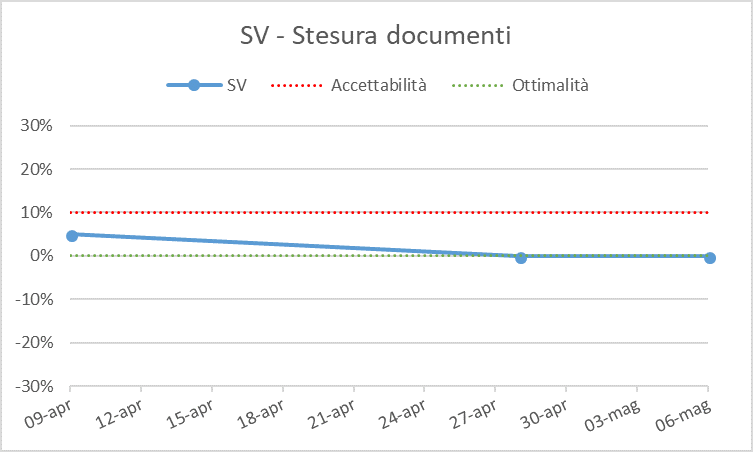
\includegraphics[scale=0.75]{img/Grafici/SV-Documenti.png}
		\caption{Schedule Variance per la stesura di ogni documento; \textcolor{green}{\checkmark} indica il raggiungimento della soglia di ottimalità, mentre \textcolor{red}{x} indica il non raggiungimento della soglia di accettabilità.}
	\label{fig:SV-Documenti}
\end{figure}

\begin{itemize}
	\item Schedule Variance finale: 0. 
	Il grafico evidenzia uno sforamento dei tempi riservati alla stesura delle \NdP{}, il quale viene però compensato da un anticipo sui tempi di stesura dello \SdF{}: il ritardo si quantifica in 2 giorni, esattamente come l'anticipo, mentre per la stesura degli altri documenti si sono rispettati i tempi previsti. 
	
	\item Soglia raggiunta: ottimalità.
\end{itemize}

\subsubsection{Cost Variance}
Il calcolo della Cost Variance sul \emph{processo di documentazione} ha portato il seguente risultato: 

{
\renewcommand{\arraystretch}{2}
\centering
\begin{tabular}{| c | c | c | c | c |}
	\hline
	\textbf{Processo} & \textbf{BCWP} & \textbf{ACWP} & \textbf{CV} & \textbf{Valutazione} \\
	\hline
	Documentazione & 3870\euro & 3840\euro & 0,78\% & Ottimale \\
	\hline
\end{tabular}

}


\subsection{Verifica dei documenti}
\subsubsection{Schedule Variance}
Nels seguente grafico vengono riportati i valori ottenuti calcolando la Schedule Variance sui tempi di verifica di ogni documento rispetto ai tempi prefissati nel \PdP{}:

\begin{figure}[h!]
	\centering
	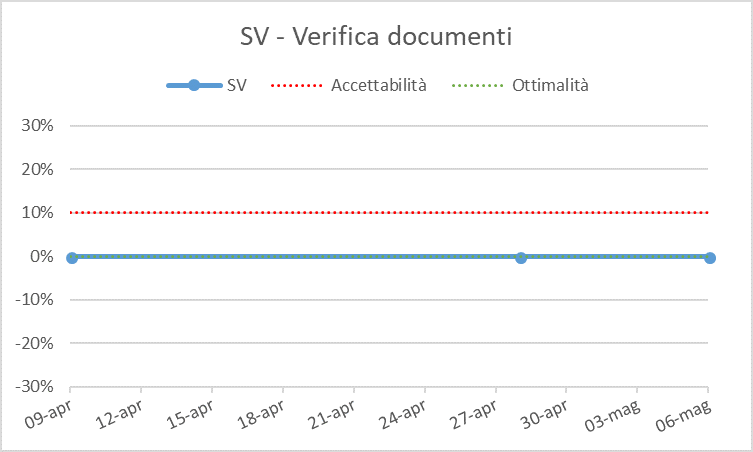
\includegraphics[scale=0.75]{img/Grafici/SV-VerDocumenti.png}
	\caption{Schedule Variance per la verifica di ogni documento; \textcolor{green}{\checkmark} indica il raggiungimento della soglia di ottimalità, mentre \textcolor{red}{x} indica il non raggiungimento della soglia di accettabilità.}
	\label{fig:SV-VerDocumenti}
\end{figure}

\begin{itemize}
	\item Schedule Variance finale: 0. 
	Il processo di verifica è stato completato senza anticipi nè ritardi;
	
	\item Soglia raggiunta: ottimalità.
\end{itemize}


\subsubsection{Cost Variance}
Il calcolo della Cost Variance sul \emph{processo di verifica} ha portato il seguente risultato: 

{
	\renewcommand{\arraystretch}{2}
	\centering
	\begin{tabular}{| c | c | c | c | c |}
		\hline
		\textbf{Processo} & \textbf{BCWP} & \textbf{ACWP} & \textbf{CV} & \textbf{Valutazione} \\
		\hline
		Verifica & 300\euro & 300\euro & 0\% & Ottimale \\
		\hline
	\end{tabular}
	
}

\newpage

\subsubsection{Errori ortografici}
Durante l'ultima verifica, sono stati rilevati all'interno dei vari documenti alcuni errori ortografici, il cui numero è specificato nel seguente grafico:

\begin{figure}[h!]
	\centering
	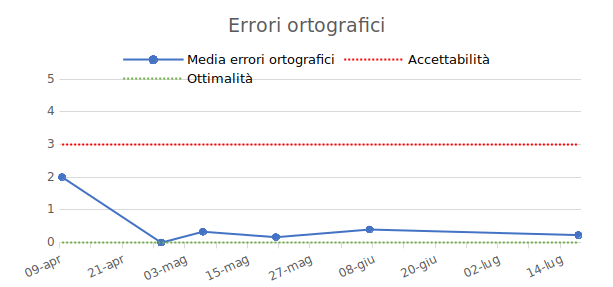
\includegraphics[scale=0.6]{img/Grafici/Errori_orto.png}
	\caption{Errori ortografici trovati in ogni documento; più il numero di errori è elevato, più ci si allontana dall'ottimalità.}
	\label{fig:Errori_orto}
\end{figure}

\begin{itemize}
\item Errori ortografici totali: 9.
\item Soglia raggiunta: con una media di 2 errori per documento, in generale si è rimasti dentro la soglia di accettabilità.
\end{itemize}

\subsubsection{Errori concettuali}

\begin{figure}[h!]
	\centering
	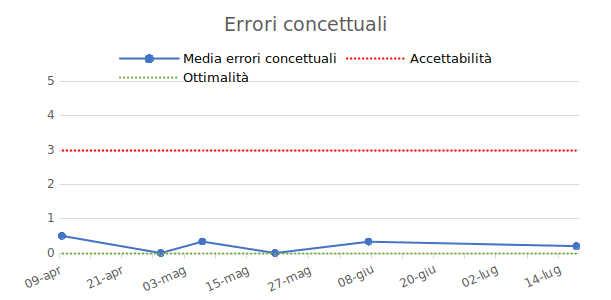
\includegraphics[scale=0.6]{img/Grafici/Errori_conce.png}
	\caption{Errori di concetto trovati in ogni documento; più il numero di errori è elevato, più ci si allontana dall'ottimalità.}
	\label{fig:Errori_conce}
\end{figure}

\begin{itemize}
	\item Errori concettuali totali: 3.
	\item Soglia raggiunta: con una media di 0,5 errori per documento, in generale si è rimasti ben dentro la soglia di accettabilità; in effetti la maggior parte dei documenti sono rimasti entro la soglia di ottimalità.
\end{itemize}

\subsubsection{Errori di forma}

\begin{figure}[h!]
	\centering
	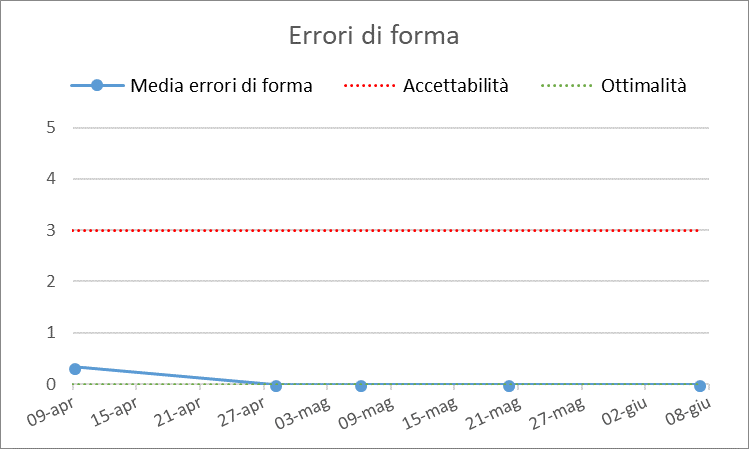
\includegraphics[scale=0.6]{img/Grafici/Errori_forma.png}
	\caption{Errori di forma trovati in ogni documento; più il numero di errori è elevato, più ci si allontana dall'ottimalità.}
	\label{fig:Errori_forma}
\end{figure}

\begin{itemize}
	\item Errori di forma totali: 3.
	\item Soglia raggiunta: con una media di 0,33 errori per documento, in generale si è rimasti ben dentro la soglia di accettabilità; in effetti la maggior parte dei documenti sono rimasti entro la soglia di ottimalità.
\end{itemize}

\newpage

\subsubsection{Indice Gulpease}

Tutti i documenti consegnati sono stati sottoposti al calcolo dell'Indice Gulpease per valutarne il grado di leggibilità, il quale è riportato nel seguente grafico:

\begin{figure}[h!]
	\centering
	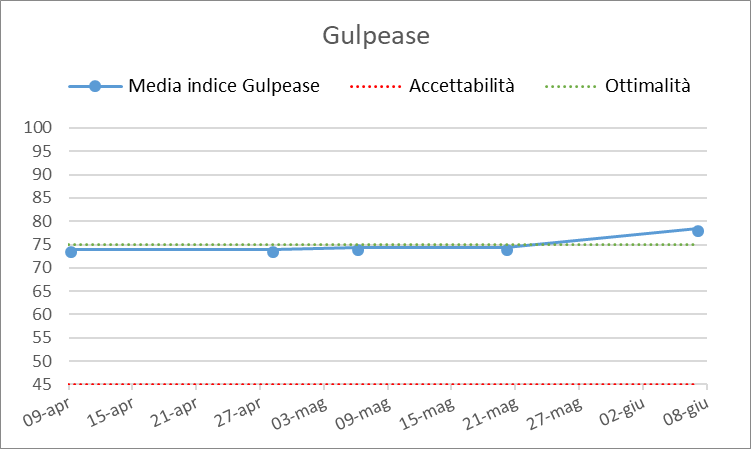
\includegraphics[scale=0.6]{img/Grafici/Gulpease.png}
	\caption{Indice Gulpease di ogni documento; più il valore è alto, più ci si avvicina all'ottimalità.}
	\label{fig:Gulpease}
\end{figure}

\begin{itemize}
	\item Soglia raggiunta: con una media di 73,84 punti, in generale si è rimasti dentro la soglia di accettabilità, arrivando poco sotto all'ottimalità.
\end{itemize}





\end{document}


